\section{Human Resource Allocation}
\label{DDHR}
The first part of the project will involve a team of five specialists designing the five critical subsystems and one person designing the orbits of the swarm. The other four members will concentrate on the development of the software that will be used to assist the trade-off and verify the design. At later stages, some of the the software engineering personnel is heavily involved in designing proper algorithms for the processing of mission data, while others will be brought in to assist with detailed design. 

A schematic representation of the resource allocation can be found in figure \ref{fig:DDBBHR} on page \pageref{fig:DDBBHR}.

\begin{figure}[h!]
\begin{center}
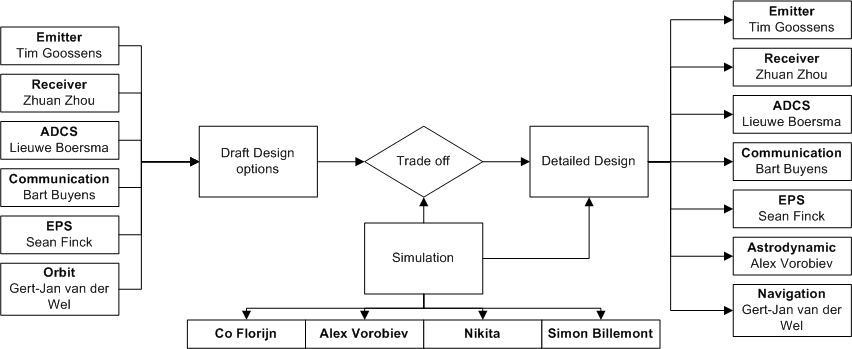
\includegraphics[width=0.9\textwidth]{chapters/img/DDBBHR.jpg}
\end{center}
\caption{Human resource allocation chart.}
\label{fig:DDBBHR}
\end{figure}

Table \ref{tab:RWD} on page \pageref{tab:RWD} indicates the allocation of tasks to each person.

\newpage
\begin{center}
\begin{longtable}{|l|l|c|c|}\hline
 Chapter & Documentation                      & Author & Checked by \\\hline\hline
 -       & Title Page                           & Alex & - \\\hline     -       & Abstract                             & Lieuwe & Tim \\\hline    
 -       & Preface                              & Co & All \\\hline
 -       & List of Symbol                       & Sean & - \\\hline\hline
 1       & Introduction                         & Bart & All \\\hline\hline
 2       & Project Management                   & - & -\\\hline
 2.1     & \ -Human Resource Allocation         & Zhuan & Sean, Nikita \\\hline
 2.2     & \ -Operations and Logistics          & GJ & Bart \\\hline
 2.3     & \ -Project Design and Development Logic & Lieuwe & Sean, Nikita \\\hline
 2.4     & \ -Project Gantt Chart               & Lieuwe & Nikita \\\hline\hline
 3       & Mission Approach                     & - & -\\\hline
 3.1     & \ -Function Flow Diagram             & Lieuwe, Zhuan & Bart \\\hline
 3.2     & \ -Function Breakdown Structure      & Lieuwe, Zhuan & Bart \\\hline
 3.3     & \ -H/W Block Diagram                 & Lieuwe, & GJ \\\hline
 3.4     & \ -S/W Block Diagram                 & Nikita & GJ \\\hline
 3.5     & \ -Electrical Block Diagram          & Sean & Bart \\\hline
 3.6     & \ -Data Handling Block Diagram       & GJ & Bart\\\hline
 3.7     & \ -Communication Block Diagram       & Bart & GJ\\\hline
 3.8     & \ -Mass Budget Breakdown             & Zhuan & Sean, Nikita \\\hline
 3.9     & \ -Cost Budget Breakdown             & Zhuan & Sean, Nikita \\\hline\hline
 4       & Risk Management                      & Tim, Zhuan & GJ \\\hline\hline
 5       & Launch and Astrodynamic Characteristics & Alex & -\\\hline
 5.1     & \ -Launch Segment                    & Alex, Sean & Co \\\hline
 5.2     & \ -Space Segment                     & Alex & Co \\\hline
 5.3     & \ -Space Environment and Shielding   & Alex & Co \\\hline\hline
 6       & Emitter Satellite                    & - & -\\\hline
 6.1     & \ -Detailed Design Optical Emitting Payload & Tim & Sean, Co \\\hline
 6.1.1   & \ \ -Principle of AlGaAs Laser Diode & Tim & Sean, Co \\\hline
 6.1.2   & \ \ -Diode Pumped Solide-State Laser Configuration & Tim & Sean, Co \\\hline
 6.1.3   & \ \ -Optical Characteristics        & Tim & Sean, Co\\\hline
 6.1.4   & \ \ -Gaussian Beam Propagation and Diffraction & Tim &  Sean, Co\\\hline  
 6.1.5   & \ \ -Thermal Control                & Tim, Lieuwe & Sean, Co\\\hline
 6.1.6   & \ \ -Laser Lifetime Expectancy     & Tim & Sean, Co\\\hline
 6.1.7   & \ \ -Laser Focus Calculation        & Zhuan & Sean, Co\\\hline
 6.2     & \ -Navigation                        & GJ & Sean \\\hline
 6.3     & \ -Communication Subsystem           & Bart & Sean\\\hline
 6.4     & \ -ADCS                              & Lieuwe & Sean\\\hline
 6.5     & \ -EPS                               & Sean & Nikita\\\hline\hline
 7       & Receiver Satellite                   & - & - \\\hline
 7.1     & \ -Detailed Design Optical Receiver Payload & Zhuan, Co & Nikita, Co\\\hline
 7.1.1   & \ \ -Introduction                           & Co & Nikita, Co\\\hline
 7.1.2   & \ \ -SPAD                           & Tim, Zhuan & Nikita, Co\\\hline
 7.1.3   & \ \ -Prism Design                   & Zhuan & Nikita, Co\\\hline
 7.1.4   & \ \ -Summary                        & Zhuan & Nikita, Co\\\hline
 7.1.5   & \ \ -Payload Cost Estimation        & Tim, Zhuan & Nikita, Co\\\hline
 7.2   & \ -Navigation                        & GJ & Nikita\\\hline
 7.3     & \ -Communication Subsystem           & Bart & Nikita\\\hline
 7.4     & \ -ADCS                              & Lieuwe & Nikita\\\hline
 7.5     & \ -EPS                               & Sean & Nikita\\\hline\hline
 8       & Data Validation                      & Simon, Co, Nikita & Nikita \\\hline
 8.1     & \ -Software Tool Internals           & Simon, Co, Nikita & Nikita \\\hline
 8.2     & \ -Validation Results                & Simon, Co, Nikita & Nikita \\\hline\hline
 9       & Sustainable Development Strategy     &Bart, Sean & GJ, Sean \\\hline\hline
 10      & Compliance Matrix                    & Sean & GJ \\\hline\hline
 11      & Conclusion and Recommendations       & Lieuwe & All\\\hline\hline
 -       & Others                               & - & - \\\hline
 -       & \ -Catia Drawing                     & Lieuwe & -\\\hline
 -       & \ -Latex Compile                     & Zhuan & -\\\hline

\caption{Report writing distribution.}
\label{tab:RWD}
\end{longtable}
\end{center}